\documentclass[12pt]{article}
\usepackage{amsmath}
\usepackage{amssymb}
\usepackage[letterpaper,top=0.75in,bottom=0.75in,left=0.75in,right=0.75in,centering]{geometry}
%\usepackage{fancyhdr}
\usepackage{enumerate}
%\usepackage{lastpage}
\usepackage{multicol}
\usepackage{graphicx}

\reversemarginpar

%\pagestyle{fancy}
%\cfoot{}
%\lhead{Math 1560}\chead{Test \# 1}\rhead{May 18th, 2017}
%\rfoot{Total: 10 points}
%\chead{{\bf Name:}}
\newcommand{\points}[1]{\marginpar{\hspace{24pt}[#1]}}
\newcommand{\skipline}{\vspace{12pt}}
%\renewcommand{\headrulewidth}{0in}
\headheight 30pt

\newcommand{\di}{\displaystyle}
\newcommand{\abs}[1]{\lvert #1\rvert}
\newcommand{\len}[1]{\lVert #1\rVert}
\renewcommand{\i}{\mathbf{i}}
\renewcommand{\j}{\mathbf{j}}
\renewcommand{\k}{\mathbf{k}}
\newcommand{\R}{\mathbb{R}}
\newcommand{\aaa}{\mathbf{a}}
\newcommand{\bbb}{\mathbf{b}}
\newcommand{\ccc}{\mathbf{c}}
\newcommand{\dotp}{\boldsymbol{\cdot}}
\newcommand{\bbm}{\begin{bmatrix}}
\newcommand{\ebm}{\end{bmatrix}}                   
                  
\begin{document}


\author{Instructor: Sean Fitzpatrick}
\thispagestyle{empty}
\vglue1cm
\begin{center}

{\bf MATH 1410 - Tutorial \#1 Solutions}
\end{center}



Additional practice problems:
\begin{enumerate}
\item Given $z=3-2i$ and $w=4+5i$, compute:

\begin{enumerate}
\item $z+w = (3-2i)+(4+5i) = 7+3i$
\item $3z-2\overline{w} = 3(3-2i)-2(4-5i)=9-8+i(-6+10)=1+4i$
\item $z^2=(3-2i)(3-2i)=9-6i-6i+4i^2=5-12i$
\item $zw=(3-2i)(4+5i)=12+15i-8i-10i^2=22+7i$
\item $\dfrac{\overline{z}}{w} = \dfrac{\overline{z}\overline{w}}{\abs{w}^2} = \frac{1}{41}(3+2i)(4-5i)=\frac{22}{41}-\frac{7}{41}i.$
\end{enumerate}


\item Compute the following powers of $i$:
\begin{enumerate}
\item $i^3=-i$ \item $i^4=1$ \item $i^6=i^2\cdot i^4=(-1)(1)=-1$ \item $i^{-5} = (-i)^5 = -i^5=-i$ (Note $i^{-1}=1/i = -i$.) \item $i^{1410} = i^{4(352)+2}=(i^4)^{352}\cdot i^2 = 1^{352}(-1)=-1.$
\end{enumerate}

\item Convert from polar to rectangular form:

\begin{enumerate}
\item $z=3e^{i(\pi/6) } = 3(\cos(\pi/6)+i\sin(\pi/6)) = 3\left(\frac{\sqrt{3}}{2}+i\frac12\right)=\frac{3\sqrt{3}}{2}+\frac32 i$. 
\item $z= 2e^{i(17\pi/4) }=2(\cos(17\pi/4)+i\sin(17\pi/4))=2\left(\frac{\sqrt{2}}{2}+i\frac{\sqrt{2}}{2}\right)=\sqrt{2}+i\sqrt{2}$.

(Note that $\frac{17\pi}{4} = \frac{16\pi}{4}+\frac{\pi}{4} = 4\pi+\frac{\pi}{4}$, so $\frac{17\pi}{4}$ is in the first quadrant.)

 \item $z=5e^{i(-19\pi/6)}=5(\cos(-19\pi/6)+i\sin(-19\pi/6))= 5\left(-1\frac12+i\frac{\sqrt{3}}{2}\right)=-\frac{5}{2}+i\frac{5\sqrt{3}}{2}$.
 
(Since the angle is negative, the rotation is clockwise. We have
\[
-\frac{19\pi}{6} = -\left(\frac{18\pi}{6}+\frac{\pi}{6}\right)=-3\pi-\frac{\pi}{6}.
\]
The rotation through $3\pi$ puts us on the negative $x$-axis, and the further clockwise rotation by $\pi/6$ puts us in the second quadrant.)

  \item $z=1410e^{i(1410\pi) }=1410(\cos(1410\pi)+i\sin(1410\pi))=1410.$
\end{enumerate}

\end{enumerate}




\newpage
%\thispagestyle{empty}
  \textbf{Assigned problems}
  \begin{enumerate}
    \item Solve the following equations for $z$:
 
    \begin{enumerate}
    \item $\dfrac{3z}{5-2z} = 1+3i$
    
    We first multiply both sides by $5-2z$ to clear the denominator:
    \[
    3z=(1+3i)(5-2z) = 5(1+3i)-2z(1+3i)=5+15i-z(2+6i).
    \]
    Next, we add $(2+6i)z$ to both sides to collect all terms involving $z$ on the left, and factor:
    \begin{align*}
    3z+(2+6i)z & = 5+15i, \tag*{so}\\
    (3+(2+6i))z & = (5+6i)z = 5+15i.
    \end{align*}
    Finally, we divide both sides by $5+6i$ to isolate $z$:
    \[
    z = \frac{5+15i}{5+6i} = \frac{(5+15i)(5-6i)}{(5+6i)(5-6i)} = \frac{25-90(-1)+75i -30i}{5^2+6^2} = \frac{115}{61}+\frac{45}{61}i.
    \]
    
    \item $3z+(2-4i)\overline{z} = 4+5i$

    Because of the presence of the complex conjugate $\overline{z}$, we need to write $z$ in terms of its real and imaginary parts. Letting $z=a+ib$, we have $\overline{z}=a-ib$. Substituting these into our equation, we have 
    \[
    3(a+ib)+(2-4i)(a-ib)=4+5i.
    \]
    Expanding the left-hand side, we get:
    \begin{align*}
    5a+3ib+2a-2ib-4ia+4b(-1) & = 4+5i\\
    (5a-4b)+i(-4a+b) & = 4+5i.
    \end{align*}
    Note that we've collected the real and imaginary parts together on the left. This allows us to compare the two sides of the equation. By definition of equality for complex numbers, the real parts on each side must be equal, and so must the imaginary parts. This gives us the pair of equations
    \[\arraycolsep=1pt
    \begin{array}{ccccc}
    5a&-&4b&=&4\\
    -4a&+&b&=&5
    \end{array}
    \]
The common solution to these two equations is $a=-\dfrac{24}{11}$ and $b=-\dfrac{41}{11}$, so our solution is
\[
z=-\frac{24}{11}-i\frac{41}{11}.
\]
(You'll learn how to solve systems of equations like this systematically later in the course. For this tutorial, arriving at the equations was good enough.)
    \end{enumerate}
      
        
  
  \end{enumerate}\pagebreak

  \begin{multicols}{2}

  \begin{enumerate}
    \addtocounter{enumi}{1}
      \item A complex number $z$ is plotted on the right. On the same set of coordinate axes, also plot:
      \begin{multicols}{2}
      \begin{enumerate}
      \item $2z$
      \item $\overline{z}$
      \item $z^2$
      \item $\dfrac{1}{z}$
      \end{enumerate}
      \end{multicols}
      Your plots do not have to be perfectly accurate and you do not have to explain your choices here, but you should be sure that you could explain them if asked to do so.
      \begin{center}
      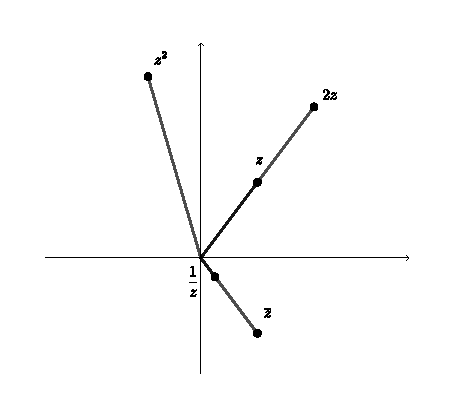
\includegraphics[width=0.8\columnwidth]{T1-2sol}
      \end{center}
  \end{enumerate}
\end{multicols}
Note: the reasoning used above is the following: given $r=2$, we know $z=2e^{i\theta}$ for some $\theta$. Then $2z=2(2e^{i\theta})=4e^{i\theta}$ is in the same direction but twice as far from the origin. We know $\overline{z}$ is a reflection across the $x$-axis. (In polar form, $\overline{z}=2e^{-i\theta}$.)
For $z^2$, we have $z^2=(2e^{i\theta})^2=2^2(e^{i\theta})^2=4e^{i(2\theta)}$, so the distance from the origin is 4, and the angle is doubled. Finally,
\[
\frac{1}{z} = \frac{1}{2e^{i\theta}}=\frac{1}{2}(e^{i\theta})^{-1}=\frac{1}{2}e^{-i\theta},
\]
so we place our point a distance of $\frac12$ from the origin, in the same direction as $\overline{z}$.

\bigskip

\begin{enumerate}
\addtocounter{enumi}{2}
\item Convert $z=1-\sqrt{3}i$ to polar form, and compute the powers $z^7$ and $z^{-3}$.

\medskip

To convert to polar form, we first compute the modulus:
\[
r=\abs{z} = \sqrt{(1)^2+(-\sqrt{3})^2} = \sqrt{1+3}=\sqrt{4}=2.
\]
We want to re-write in the form $z=r(\cos\theta+i\sin\theta)$. We have
\[
z=1-\sqrt{3}i = 2\left((\frac{1}{2}+i\left(-\frac{\sqrt{3}}{2}\right)\right),
\]
so we're looking for an angle $\theta$ with $\cos\theta = 1/2$ and $\sin\theta=-\sqrt{3}/2$. Looking at our unit circle, we see that $\theta = -\pi/3$ does the trick. (Or $\theta = 5\pi/3$ if you prefer an angle in $[0,2\pi)$.) Thus,
\[
z = 2(\cos(-\pi/3)+i\sin(-\pi/3)) = 2e^{i(-\pi/3)}.
\]

Now that $z$ is in polar form, the powers are straight-forward:
\[
z^7 = (2e^{i(-\pi/3)})^7 = 2^7(e^{i(-\pi/3)})^7 = 128e^{i(-7\pi/3)}.
\]
If you wish to convert back to rectangular form, note that $-7\pi/3 = -2\pi-\pi/3$, so our angle is equivalent to the one we started with, giving
\[
z^7=128\left(\frac12+i\left(-\frac{\sqrt{3}}{2}\right)\right) = 64-64\sqrt{3}i.
\]
Similarly,
\[
z^{-3} = (2e^{i(-\pi/3)})^{-3} = 2^{-3}(e^{i(-\pi/3)})^{-3} = \frac{1}{8}e^{i\pi} = -\frac18.
\]
\end{enumerate}
  
\end{document}